\documentclass[10pt,a4paper]{article}
\usepackage[margin=2.2cm]{geometry}
\usepackage[T1]{fontenc}
\usepackage{lmodern}
\usepackage{amsmath}
\usepackage{booktabs}
\usepackage{graphicx}
\usepackage{multirow}
\usepackage[numbers,sort&compress]{natbib}
\usepackage{xcolor}
\usepackage[hidelinks]{hyperref}
\usepackage{xurl}

\title{When the Channel Changes: Layer Choice, Calibration Transfer and a Padding Pitfall in Frozen-WavLM Speech Deepfake Detection}
\author{Muzammal Hussain\\
\small Independent researcher, Glasgow, United Kingdom\\
\small ORCID: \href{https://orcid.org/0009-0001-2570-5686}{0009-0001-2570-5686}}
\date{}

\begin{document}
\maketitle

\begin{abstract}
Speech deepfake detectors are usually reported by their equal error rate (EER) on clean benchmark audio, while the
people who would use them hear speech through phone lines, codecs and messaging apps. We train light classifiers on
frozen WavLM Base+ features from ASVspoof 2019 LA and study what happens when only the channel changes. Across four
hidden layers, two classifiers, three classifier seeds and four conditions (clean, a simulated narrow-band phone
line, the same line with 15\,dB noise, and Opus at 16\,kbps), the choice of layer matters more than the classifier:
layer 6 with a small MLP keeps a mean EER of 1.7\%, 2.2\% and 2.1\% on clean, phone and Opus audio, and 8.1\% with
noise, where layers 3 and 12 reach 23.6\% and 27.0\%. On the out-of-domain In-the-Wild dataset (31,779 clips) the
same model reaches 18.0\% EER and keeps the best ranking of layers. Calibration fitted on clean development data does
not transfer: Cllr exceeds 1 bit in 5 of 8 WavLM models with noise and in 7 of 8 on In-the-Wild, while minCllr shows
that the scores still separate the classes. With the threshold fixed on development data, the dominant error on
In-the-Wild is real speech called fake (30.7\% of real clips against 7.0\% of fakes missed). We also document how
zero-padding inside a batch changes WavLM Base+ features through its group-normalised first convolution: for clips
shorter than 2\,s, the log-likelihood ratio moved by 2.98 on average and 11\% of three-way verdicts changed. Code,
result files and a browser demo are public.
\end{abstract}

\section{Introduction}
Cloned and synthetic voices can be used to impersonate relatives, colleagues and officials over the phone. A
countermeasure that is useful in that setting has to work on audio that has passed through a telephone network, a
voice-over-IP codec or a messaging app, and it has to say how sure it is. Benchmarks such as ASVspoof 2019 LA
\cite{wang2020asvspoof} are recorded and distributed as clean wide-band audio, and most results are summarised by the
EER, which needs no decision threshold and says nothing about calibration.

Self-supervised speech models are now the standard front end for spoofing countermeasures
\cite{wang2022investigating,tak2022automatic}, and frozen representations with a simple classifier can generalise
well and be reasonably calibrated \cite{pascu2024towards}. Which hidden layer to use has been analysed in detail
\cite{elkheir2025comprehensive}, and channel effects are part of recent challenges and benchmarks
\cite{liu2023asvspoof,wang2026asvspoof5,shi2025benchmarking}. This paper does not propose a new model. It asks a
narrower, practical question about one cheap and common recipe---frozen WavLM Base+ \cite{chen2022wavlm} features with
a logistic regression or a small MLP---when nothing changes except the channel:
\begin{enumerate}
\item How does the choice of hidden layer interact with telephone filtering, noise and a low-bitrate codec, measured
over several classifier seeds, and does the ranking hold on real out-of-domain audio?
\item Does a calibration fitted on clean development data remain valid after the channel changes?
\item What kind of error does a fixed threshold make on real-world audio?
\item How large is the effect of zero-padding inside a batch on the scores and verdicts of a deployed detector?
\end{enumerate}
Our contributions are a controlled, seed-repeated measurement of these four points, with discrimination (EER,
minCllr) and calibration (Cllr) reported separately \cite{brummer2006application}; an out-of-domain check on
In-the-Wild \cite{muller2022does} with a threshold fixed in advance; a documented measurement of the padding effect
by clip length; and a public browser demo whose informal behaviour on real phone and messaging-app recordings is
consistent with the measured error pattern. None of these ingredients is new on its own; the value of the study is in
measuring them together on one pipeline and reporting where it fails.

\section{Related work}
\textbf{Self-supervised front ends.} Wang and Yamagishi \cite{wang2022investigating} showed that pre-trained
wav2vec~2.0 and HuBERT front ends outperform signal-processing features for spoofing countermeasures, especially when
fine-tuned. Tak et al. \cite{tak2022automatic} combined a fine-tuned XLS-R front end with AASIST and data
augmentation. Pascu et al. \cite{pascu2024towards} found that large frozen representations with logistic regression
generalise across eight datasets and give more reliable probabilities than earlier models. Our setup is close to
theirs but uses a small model (WavLM Base+) and studies channel shift rather than dataset shift alone.

\textbf{Layer-wise analysis.} El Kheir et al. \cite{elkheir2025comprehensive} analysed wav2vec~2.0, HuBERT and WavLM
layer by layer across languages and deepfake types and found that lower layers carry the most discriminative
information, so a reduced number of layers is often sufficient. We do not repeat that analysis; we ask how single
layers behave when the channel changes.

\textbf{Channels and real-world data.} ASVspoof 2021 LA introduced telephony and transmission codecs
\cite{liu2023asvspoof}, and ASVspoof 5 applies eleven codec conditions, including narrow-band ones, to its evaluation
data \cite{wang2026asvspoof5}. Shi et al. \cite{shi2025benchmarking} benchmark robustness to codecs and packet loss in
communication scenarios. M\"uller et al. \cite{muller2022does} released In-the-Wild and showed that models trained on
ASVspoof degrade sharply on found audio; later work attributes much of the gap to differences in generation methods
\cite{muller2024harder}.

\textbf{Calibration and thresholds.} Cllr and its minimum over monotonic recalibrations separate discrimination from
calibration \cite{brummer2006application}. A recent preprint shows that a low in-domain EER can hide a large failure
when a threshold is transferred to another domain \cite{zhou2026eer}. Our results agree with that observation for a
frozen-feature detector and add the direction of the error.

\textbf{Padding.} For wav2vec~2.0-style models with group normalisation in the first convolution, padded and unpadded
inputs give different outputs; this is known among practitioners \cite{hf2023padding}. We measure its effect on
deepfake scores and verdicts.

\section{Experimental setup}
\subsection{Data}
We use the logical-access part of ASVspoof 2019 \cite{wang2020asvspoof}. Classifiers are trained on all 25,380
training clips (attacks A01--A06). Calibration uses a fixed sample of 2,020 development clips (1,000 bona fide and up
to 170 per attack). Evaluation uses a stratified sample of 9,800 clips: 2,000 bona fide and 600 per attack A07--A19,
drawn with seed 42; all clip identifiers are published. A16 and A19 reuse the A04 and A06 algorithms, so we also
report an EER on the eleven unseen attacks. Training, development and evaluation speakers are disjoint by design of
the corpus.

For the out-of-domain test we use all 31,779 clips of In-the-Wild \cite{muller2022does} (19,963 bona fide, 11,816
spoof, 54 speaker labels in the metadata), downloaded from the authors' release. Nothing is trained or tuned on it.
All clips are 16\,kHz; their mean length is 4.29\,s and their median 3.27\,s, so 61\% of them are shorter than the
4\,s window used below.

\subsection{Channel conditions}
Training uses clean audio only. Each evaluation clip is scored in four conditions: \emph{clean}; \emph{phone line}
(resampled to 8\,kHz, band-limited to 300--3400\,Hz, G.711-style $\mu$-law companding \cite{itu1988g711}, and back to
16\,kHz); \emph{phone + noise} (white noise at 15\,dB SNR added before the same line); and \emph{Opus 16\,kbps} (encoded and
decoded with ffmpeg/libopus in VoIP mode \cite{rfc6716}). The conditions are simulated; Section~\ref{sec:case}
compares them with a few real recordings.

\subsection{Features and classifiers}
Each clip is cut to its first 4\,s, passed through the channel condition and normalised to zero mean and unit variance. We extract hidden states 3, 6, 9
and 12 of the frozen WavLM Base+ model \cite{chen2022wavlm} (float16 on GPU) and mean-pool them over frames, giving
a 768-dimensional vector per layer. As an acoustic baseline we use the mean and standard deviation of 40 MFCCs.
Each feature set feeds two classifiers after standardisation: logistic regression with balanced class weights, and an
MLP with one hidden layer of 256 units, early stopping and L2 penalty $10^{-3}$. The MLP is trained with classifier
seeds 42, 43 and 44 on the same clips and features; logistic regression is deterministic.

Clips in a batch are grouped by exact length, so no clip is zero-padded (Section~\ref{sec:padding} explains why).

\subsection{Calibration and metrics}
A raw classifier score $p$ is mapped to a log-likelihood ratio $\ell = a\,\mathrm{logit}(p) + b$ by logistic
regression on the development set with equal total weight for each class, so that the map does not absorb the class
mix of the development sample. A posterior for any stated spoof prior $\pi$ is $\sigma(\ell + \mathrm{logit}\,\pi)$.
We report the EER (with a bootstrap 95\% interval in the released tables), the ROC AUC, and
\begin{equation}
C_\mathrm{llr} = \frac{1}{2\ln 2}\left[\frac{1}{N_s}\sum_{i\in s}\ln\!\left(1+e^{-\ell_i}\right)
+ \frac{1}{N_b}\sum_{j\in b}\ln\!\left(1+e^{\ell_j}\right)\right],
\end{equation}
in bits, where $s$ and $b$ are the spoof and bona fide trials \cite{brummer2006application}. A system that always
outputs $\ell=0$ has $C_\mathrm{llr}=1$; larger values mean the scores are worse than no evidence. $\min C_\mathrm{llr}$
is the same cost after the best monotonic recalibration (pool-adjacent-violators) and measures discrimination only.
We also report the expected calibration error (ECE, 15 bins) \cite{guo2017calibration} and compare our calibrator
with Platt scaling \cite{platt1999probabilistic}. Unless a single seed is stated, numbers are means over the three
classifier seeds.

For In-the-Wild we add two threshold-based views. First, the threshold is fixed at the EER point of the ASVspoof
development scores and both error rates are measured. Second, we apply the rule of our public demo: a clip is shown
as ``likely AI-generated'' if $\sigma(\ell)\ge 0.95$, ``likely real'' if $\sigma(\ell)\le 0.05$ and ``uncertain''
otherwise (an even prior).

\section{Results}
\subsection{Layer choice under channel shift}
Table~\ref{tab:eer} and Figure~\ref{fig:layers} show the EER of every model. On clean audio, layers 3 and 6 are
close (2.1\% and 1.7\% with the MLP). The phone line separates them: layer 3 rises to 6.9\% while layer 6 stays at
2.2\%. With noise, layers 3 and 12 reach 23.6\% and 27.0\% while layers 6 and 9 stay at 8.1\% and 8.9\%. Layer 6 with
the MLP is the most stable model in every condition, and its EER on the eleven unseen attacks follows the same pattern
(1.4\%, 1.6\%, 7.4\% and 1.8\%). The MFCC baseline collapses on the phone line (40.6--50.3\%), where the best WavLM
features barely move.

Opus at 16\,kbps costs little on this data: layer 6 with the MLP goes from 1.7\% to 2.1\%. The noisy phone line is
the hardest condition for every model. Single MLP runs can mislead under noise: across the three seeds, layer 12
ranged from 23.1\% to 32.6\% and layer 3 from 22.1\% to 24.6\%, whereas layer 6 stayed between 6.8\% and 9.5\%.

On In-the-Wild, every model degrades sharply, but the ranking holds. Layer 6 is the best layer with either classifier
(18.0\% and 18.1\%), layers 9 and 12 reach 23--29\%, and the MFCC models are worse than chance (AUC 0.29 and 0.44),
which means they rank real clips as more fake than the fakes. Layer 3 with the MLP is competitive on average (20.7\%)
but varies most across seeds (sd 3.5 points).

\begin{table}[t]
\centering
\caption{EER (\%) of models trained on clean ASVspoof 2019 LA. Mean over classifier seeds 42--44 with the standard
deviation in brackets (logistic regression is deterministic). ASVspoof: 9,800 evaluation clips; In-the-Wild: 31,779
clips, not used for training or calibration.}
\label{tab:eer}
\small
\begin{tabular}{llccccc}
\toprule
Features & Classifier & Clean & Phone line & Phone + noise & Opus 16\,kbps & In-the-Wild \\
\midrule
MFCC & LogReg & 19.7 & 50.3 & 37.3 & 15.3 & 66.1 \\
MFCC & MLP & 16.3 (1.1) & 40.6 (3.5) & 50.8 (0.8) & 13.4 (0.7) & 56.0 (0.7) \\
\midrule
WavLM L3 & LogReg & 3.7 & 13.5 & 24.2 & 4.7 & 32.5 \\
WavLM L3 & MLP & 2.1 (0.4) & 6.9 (2.2) & 23.6 (1.3) & 2.5 (0.4) & 20.7 (3.5) \\
WavLM L6 & LogReg & 2.6 & 3.2 & 10.5 & 3.3 & 18.1 \\
WavLM L6 & MLP & \textbf{1.7} (0.3) & \textbf{2.2} (0.1) & \textbf{8.1} (1.4) & \textbf{2.1} (0.3) & \textbf{18.0} (1.5) \\
WavLM L9 & LogReg & 3.8 & 4.6 & 12.2 & 4.0 & 24.6 \\
WavLM L9 & MLP & 3.5 (0.1) & 5.8 (0.3) & 8.9 (0.8) & 3.7 (0.1) & 25.4 (0.4) \\
WavLM L12 & LogReg & 5.2 & 13.2 & 39.3 & 4.6 & 23.0 \\
WavLM L12 & MLP & 5.6 (0.1) & 6.0 (0.4) & 27.0 (5.0) & 5.6 (0.1) & 29.1 (1.0) \\
\bottomrule
\end{tabular}
\end{table}

\begin{figure}[t]
\centering
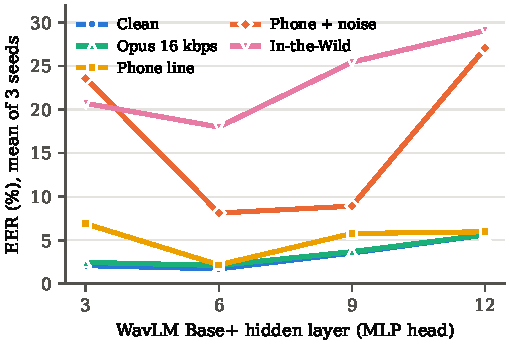
\includegraphics[width=0.62\linewidth]{figures/eer_by_layer.pdf}
\caption{EER by WavLM Base+ layer with the MLP classifier (mean of three seeds). The clean and Opus curves overlap;
exact values are in Table~\ref{tab:eer}.}
\label{fig:layers}
\end{figure}

\subsection{Calibration does not transfer}
Table~\ref{tab:cllr} separates calibration from discrimination. On clean audio every WavLM model is well below
1 bit. With noise, Cllr exceeds 1 for 5 of the 8 WavLM models (all except layer 6 with either classifier and layer 9
with the MLP), and over all 40 model--condition pairs on ASVspoof it does so in 11. minCllr stays much lower: for
layer 12 with the MLP under noise, Cllr is 3.59 against a minCllr of 0.57. The scores still rank the clips, but the
map from scores to evidence, fitted on clean development audio, is far too confident on the noisy line.

On In-the-Wild, Cllr exceeds 1 for 7 of the 8 WavLM models; only layer 3 with the MLP stays just below (0.96). Layer 6
has the lowest minCllr (0.59 with both classifiers) but Cllr of 1.33 and 1.38. In terms of the posterior at the true
spoof share of In-the-Wild (0.37), layer 3 with the MLP has the lowest ECE (0.114), followed by layer 6 with the MLP
(0.162). Comparing calibrators on ASVspoof (seed 42), the equal-weight LLR map gave a lower ECE than Platt scaling
fitted on the same development data in 25 of 40 pairs.

\begin{table}[t]
\centering
\caption{Cllr / minCllr in bits (mean of three seeds). Cllr above 1 means the calibrated scores are worse than
answering ``no evidence''; the gap to minCllr is the calibration loss.}
\label{tab:cllr}
\small
\begin{tabular}{llccccc}
\toprule
Features & Classifier & Clean & Phone line & Phone + noise & Opus 16\,kbps & In-the-Wild \\
\midrule
MFCC & LogReg & 0.74 / 0.61 & 3.29 / 0.98 & 1.40 / 0.89 & 1.66 / 0.47 & 3.77 / 1.00 \\
MFCC & MLP & 0.74 / 0.52 & 2.13 / 0.93 & 2.38 / 1.00 & 0.97 / 0.45 & 2.31 / 1.00 \\
\midrule
WavLM L3 & LogReg & 0.48 / 0.14 & 0.61 / 0.43 & 3.36 / 0.71 & 0.29 / 0.17 & 2.14 / 0.87 \\
WavLM L3 & MLP & 0.17 / 0.08 & 0.27 / 0.24 & 1.48 / 0.69 & 0.11 / 0.10 & 0.96 / 0.65 \\
WavLM L6 & LogReg & 0.21 / 0.10 & 0.27 / 0.12 & 0.69 / 0.35 & 0.13 / 0.11 & 1.33 / 0.59 \\
WavLM L6 & MLP & 0.21 / 0.07 & 0.13 / 0.09 & 0.70 / 0.30 & 0.11 / 0.08 & 1.38 / 0.59 \\
WavLM L9 & LogReg & 0.21 / 0.14 & 0.35 / 0.18 & 1.70 / 0.37 & 0.19 / 0.15 & 2.56 / 0.74 \\
WavLM L9 & MLP & 0.25 / 0.14 & 0.36 / 0.22 & 0.98 / 0.32 & 0.19 / 0.14 & 2.22 / 0.77 \\
WavLM L12 & LogReg & 0.28 / 0.19 & 1.29 / 0.38 & 3.26 / 0.43 & 0.21 / 0.17 & 3.09 / 0.72 \\
WavLM L12 & MLP & 0.42 / 0.21 & 0.40 / 0.23 & 3.59 / 0.57 & 0.35 / 0.20 & 3.30 / 0.83 \\
\bottomrule
\end{tabular}
\end{table}

\subsection{Thresholds on real-world audio: real speech is called fake}
Table~\ref{tab:itw} fixes the decision before seeing In-the-Wild. At the ASVspoof development EER threshold, the
errors are strongly one-sided: layer 6 with the MLP calls 30.7\% of real clips fake but misses only 7.0\% of fakes;
layers 9 and 12 call 70--93\% of real clips fake while missing at most 4.5\% of fakes. Only layer 3 with the MLP has
balanced errors (14.3\% and 21.7\%). Under the demo rule, the published model (layer 6, MLP, seed 42) shows 15.7\%
of real clips as likely AI-generated, 34.6\% as uncertain and 49.7\% as likely real; it shows 83.2\% of fakes as
likely AI-generated and 2.9\% as likely real. For a detector trained on clean studio-quality corpora, the cost of a
new domain thus falls mostly on genuine speakers.

\begin{table}[t]
\centering
\caption{In-the-Wild with decisions fixed in advance (seed 42). Left: threshold at the ASVspoof development EER
point. Right: the three-way demo rule ($\sigma(\ell)\ge0.95$ fake, $\le0.05$ real, else uncertain). All values in \%.}
\label{tab:itw}
\small
\begin{tabular}{llccc@{\hspace{1.2em}}ccc@{\hspace{1.2em}}cc}
\toprule
& & \multicolumn{3}{c}{Dev EER threshold} & \multicolumn{3}{c}{Real clips shown as} & \multicolumn{2}{c}{Fake clips shown as} \\
Features & Classifier & Real$\to$fake & Fake$\to$real & HTER & fake & uncertain & real & fake & real \\
\midrule
MFCC & MLP & 99.1 & 2.0 & 50.5 & 92.4 & 7.6 & 0.0 & 87.2 & 0.2 \\
WavLM L3 & MLP & 14.3 & 21.7 & 18.0 & 4.8 & 30.3 & 64.8 & 51.3 & 5.7 \\
WavLM L6 & LogReg & 35.8 & 7.3 & 21.5 & 21.6 & 38.4 & 40.0 & 85.1 & 2.6 \\
WavLM L6 & MLP & 30.7 & 7.0 & 18.8 & 15.7 & 34.6 & 49.7 & 83.2 & 2.9 \\
WavLM L9 & MLP & 70.3 & 4.5 & 37.4 & 44.4 & 45.3 & 10.3 & 87.2 & 0.9 \\
WavLM L12 & LogReg & 93.1 & 0.2 & 46.6 & 84.2 & 12.7 & 3.2 & 98.9 & 0.1 \\
WavLM L12 & MLP & 92.0 & 0.4 & 46.2 & 77.4 & 19.9 & 2.7 & 97.5 & 0.1 \\
\bottomrule
\end{tabular}
\end{table}

\subsection{Zero padding changes WavLM Base+ features}
\label{sec:padding}
WavLM Base+ applies group normalisation over time after its first convolution, so the statistics of a padded clip
include the padded zeros \cite{hf2023padding}. An earlier version of our pipeline padded every clip to the longest
clip of its batch of 48. We found the effect while checking the browser demo, which scores one unpadded clip at a
time, against the experiment features on 920 evaluation clips (400 bona fide and 40 per attack). Figure~\ref{fig:pad}
shows that the gap grows as clips get shorter: the mean absolute LLR difference was 0.01 for clips cut at 4\,s (never
padded), 0.41 for 3--4\,s, 1.07 for 2--3\,s and 2.98 below 2\,s, and the three-way verdict agreed on 100\%, 99.1\%,
96.8\% and 89.0\% of them. After switching to batches of equal length, the demo and the experiments agreed on every
verdict and the mean difference was about 0.01 in every length group. The headline numbers moved by at most a few
points (layer 6 with the MLP, clean, seed 42: 1.8\% before and 2.1\% after), and the conclusions above hold in both
versions. The issue matters more for real-world data: 61\% of In-the-Wild clips are shorter than 4\,s and would have
been padded.

\begin{figure}[t]
\centering
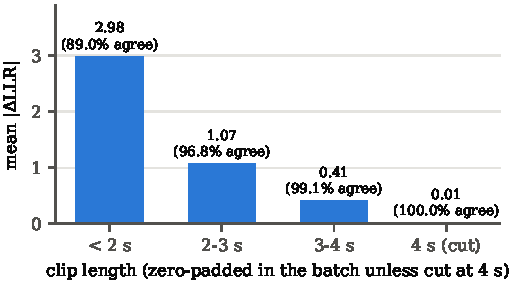
\includegraphics[width=0.62\linewidth]{figures/padding_effect.pdf}
\caption{Effect of batch zero-padding on the layer 6 + MLP detector: mean absolute LLR difference between padded
batch features and single unpadded clips, and agreement of the three-way verdict, by clip length (920 clips).}
\label{fig:pad}
\end{figure}

\subsection{Informal case study: a public demo on real recordings}
\label{sec:case}
The layer 6 + MLP model runs in a public static web page that scores audio in the browser
(see Code and data availability). We checked it informally on a handful of recordings by the author; these are anecdotes,
not a benchmark. With the model of the padded pipeline, the author's voice recorded on a laptop microphone scored
0.3\% AI probability, a genuine English WhatsApp voice note uploaded as a file scored 97.4\%, and the same note played
through a loudspeaker and recorded again scored 99.9\%. With the corrected pipeline, the same WhatsApp file scored
93.6\% (``uncertain''), a new replayed recording 95.5\% (``likely AI-generated'') and a new laptop recording 0.0\%.
Because a 16\,kbps Opus round trip alone barely affects the detector (Table~\ref{tab:eer}), the simulated codec does
not explain these false alarms; device, app processing and loudspeaker replay are other differences. The behaviour
matches the one-sided error measured on In-the-Wild.

\section{Discussion and limitations}
Three practical lessons follow. First, a layer that is best on clean data is not necessarily robust: layers 3 and 6
are close on clean audio but differ by a factor of three on the phone line, and layer 6 also transfers best to
In-the-Wild. Second, calibration should be checked under the target channel: minCllr shows that much of the loss
under shift is calibration, which could in principle be repaired with a small amount of matched data, whereas a clean
EER says nothing about it. Third, the first failure that users meet is a false alarm on genuine speech, which argues
for an explicit ``uncertain'' outcome and for reporting both error rates at a fixed threshold.

The study has clear limits. It uses one training corpus, in English, and one small front end. The channel conditions
are simulated, and white noise is a crude model of real background noise. Training uses clean audio only, without
codec or noise augmentation, which is deliberate here but known to help \cite{tak2022automatic}. Three classifier
seeds give only a rough spread and do not cover variation from the clip sample or feature extraction. In-the-Wild
differs from ASVspoof in speakers, recording conditions and generation methods at once, so our results do not
isolate the cause of the drop \cite{muller2024harder}. The case study is a handful of clips. Finally, all clips are
cut to 4\,s, while longer inputs can help \cite{muller2022does}.

\section{Conclusion}
For a frozen WavLM Base+ detector trained on ASVspoof 2019 LA, the middle layer (6) was the most robust to a
simulated phone line, noise and Opus, and also the best on In-the-Wild, where it reached 18.0\% EER. Calibration
fitted on clean data did not survive the change of channel or domain, and at a fixed threshold the errors fell mostly
on real speakers. Batch zero-padding silently changed scores of short clips. Reporting Cllr with minCllr, both error
rates at a fixed threshold, and checking that a deployed model reproduces the evaluated one are cheap steps that
would have exposed all of these issues.

\section*{Code and data availability}
Code, tests, Kaggle notebooks, clip identifiers and all result files:
\url{https://github.com/MHKhan50/voiceguard-crosslingual-audio-deepfake-detection}. Browser demo:
\url{https://huggingface.co/spaces/MHkhan50/voiceguard-fake-voice-check}. ASVspoof 2019 and In-the-Wild are used
under their own licences and are not redistributed. Experiments ran on Kaggle GPU notebooks (37.5 minutes for the
ASVspoof run, 12.9 minutes for In-the-Wild with cached ASVspoof features).

\bibliographystyle{unsrtnat}
\bibliography{references}

\end{document}
